\documentclass[12pt]{article}
\usepackage{amsmath}
\usepackage{amsmath,amssymb}
\usepackage{wrapfig}
\usepackage{graphicx}
\usepackage[margin=1in,top=0.5in]{geometry}
\usepackage{multicol}
\setlength{\columnseprule}{0.4pt}
\graphicspath{{./images/}}

\begin{document}
\title{Reinforcement Learning Threshold Assignment}
\author{220152703}
\date{}
\maketitle

\section{The SARSA Algorithm}
\begin{multicols}{2}

We can model the robot's decision-making process with a Markov Decision Process (MDP), with:

\begin{itemize}
    \item A set of states \( S \) representing the possible positions the robot can have.
    \item A set of actions \( A \) available to the robot.
    \item A transition probability function \( P(s' \mid s,a) \) that defines the likelihood of moving to state \( s' \) after taking action \( a \) in state \( s \).
    \item A reward function \( R(s,a,s') \) specifying the immediate reward received when taking action \( a \) in state \( s \) and transitioning to \( s' \).
\end{itemize}


The robot starts from a state \( s \) with the goal of selecting actions that maximise the expected return. The agent selects actions according to a policy \( \pi(a \mid s) \).

The total return the agent receives is defined as:
\[
G_t = R_{t+1} + \gamma R_{t+2} + \gamma^2 R_{t+3} + \dots
\]
\[
G_{t+1} = R_{t+2} + \gamma R_{t+3} + \dots
\]
\[
\Rightarrow G_t = R_{t+1} + \gamma G_{t+1}
\]

We denote the expected return of taking an action \( a \) in state \( s \) as \( q^\pi(s,a) \) defined as:
\[
q^\pi(s,a) = \mathbb{E}_\pi[G_t \mid S_t = s, A_t = a]
\]

This is equivalent to:
\[
q^\pi(s,a) = \mathbb{E}_\pi[R_{t+1} + \gamma q^\pi(S_{t+1}, A_{t+1}) \mid S_t = s, A_t = a]
\]

\[
\Rightarrow \mathbb{E}_\pi[R_{t+1} + \gamma q^\pi(s', a') - q^\pi(s, a) \mid S_t = s, A_t = a] = 0
\]

To maximise expected return in any state, the robot should choose the action that maximises \( q^\pi(s, a) \). Since the true values of \( q^\pi(s,a) \) are unknown, we introduce a parameterised function \( Q(s,a) \) to estimate them. The expectation then becomes approximately zero:
\[
\mathbb{E}_\pi[R_{t+1} + \gamma Q(s', a') - Q(s, a) \mid S_t = s, A_t = a] \approx 0
\]

We define a squared loss function around this quantity to make it minimizable:
\[
L(s,a) = \frac{1}{2}(Q(s,a) - (r + \gamma Q(s', a')))^2
\]

Assuming \( Q(s', a') \) is known and fixed, the partial derivative of the loss function with respect to \( Q(s,a) \) is:
\[
\frac{\partial L(s,a)}{\partial Q(s,a)} = Q(s,a) - (r + \gamma Q(s', a'))
\]

To update \( Q(s,a) \), we apply the online update rule:
\[
Q(s,a) \leftarrow Q(s,a) + \eta (r + \gamma Q(s',a') - Q(s,a))
\]
\end{multicols}

\clearpage
\textbf{Algorithm:}

\large
\begin{enumerate}
    \item Initialise \( Q(s,a) \) arbitrarily for all \( s \in S \), \( a \in A \).
    \item For each episode:
    \begin{enumerate}
        \item Initialise state \( s \)
        \item Choose action \( a \) from \( s \) using a policy derived from \( Q \)
        \item For each step of the episode:
        \begin{enumerate}
            \item Take action \( a \), observe reward \( r \) and next state \( s' \)
            \item If \( s' \) is terminal:
            \begin{itemize}
                \item Update \( Q(s,a): Q(s,a) \leftarrow Q(s,a) + \eta(r - Q(s,a)) \)
                \item Break
            \end{itemize}
            \item Choose action \( a' \) from \( s' \) using a policy derived from \( Q \)
            \item Update \( Q(s,a): Q(s,a) \leftarrow Q(s,a) + \eta (r + \gamma Q(s',a') - Q(s,a)) \)
            \item Update state and action: \( s \leftarrow s', a \leftarrow a' \)
        \end{enumerate}
    \end{enumerate}
\end{enumerate}
\normalsize

\large
\section{Training}
Two different environments were used for training. The environments we both (9*13) grids, with cliffs of reward -100, and impassable walls. Environment 1 had one reward of 5000 at (1,2). Environment 2 had that reward as well as another at (8, 11) with value 250.

Multiple training runs were completed in order to maximise the agent’s expected return, with varying hyperparameters and policies.
\clearpage

Initially, the SERSA algorithm with epsilon-greedy policy was used on the simpler 1 reward environment.
\vspace{10pt}


\begin{wrapfigure}{l}{0.6\textwidth}
  \centering
\begin{minipage}{.28\textwidth}
  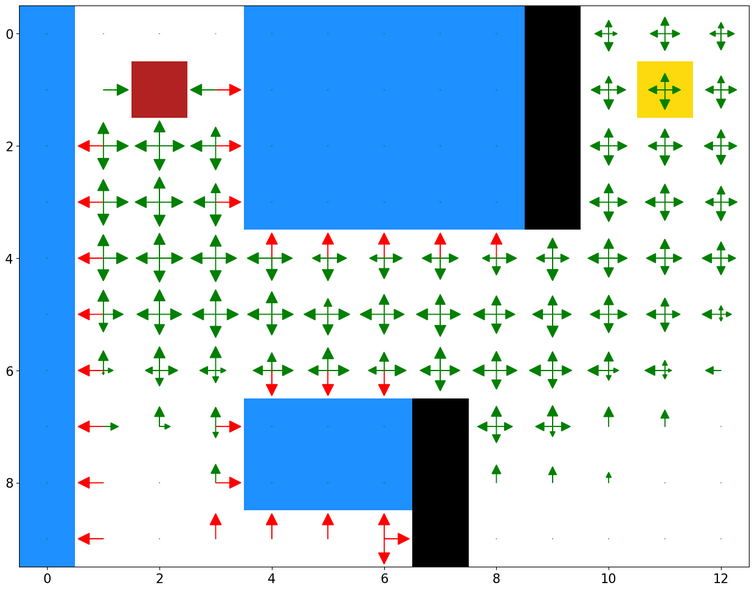
\includegraphics[width=0.9\textwidth]{1 Q plot.png}
  \caption{  num episodes = 5000, $\eta$= 0.5, $\gamma$ = 1 - 0.01, $\epsilon$ = 0.1}
\end{minipage}%
\begin{minipage}{.32\textwidth}
  \centering
  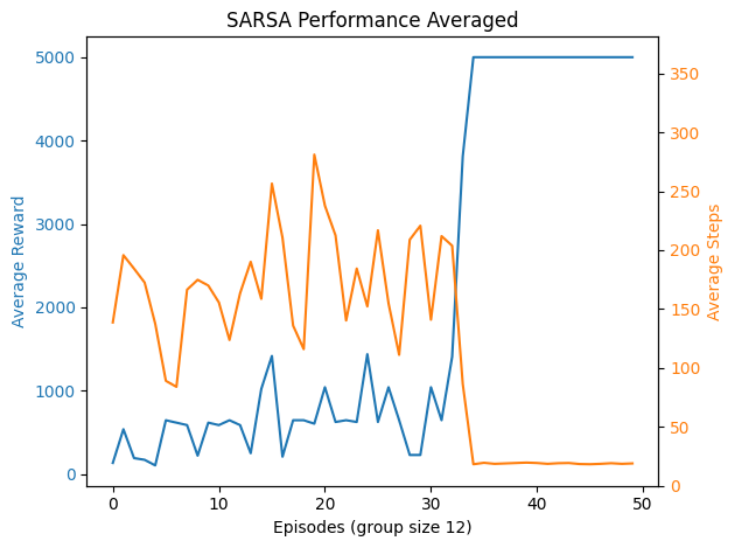
\includegraphics[width=1\textwidth]{10 performance plot.png}
\end{minipage}
\end{wrapfigure}

With these parameters SERSA very quickly learned the optimal path. $\gamma$ is set very close to 1 so that the agent cares about actions it takes far into the future (like when it is at the far reward).
\\ \\ \\

\begin{wrapfigure}{r}{0.6\textwidth}
  \centering
\begin{minipage}{.28\textwidth}
  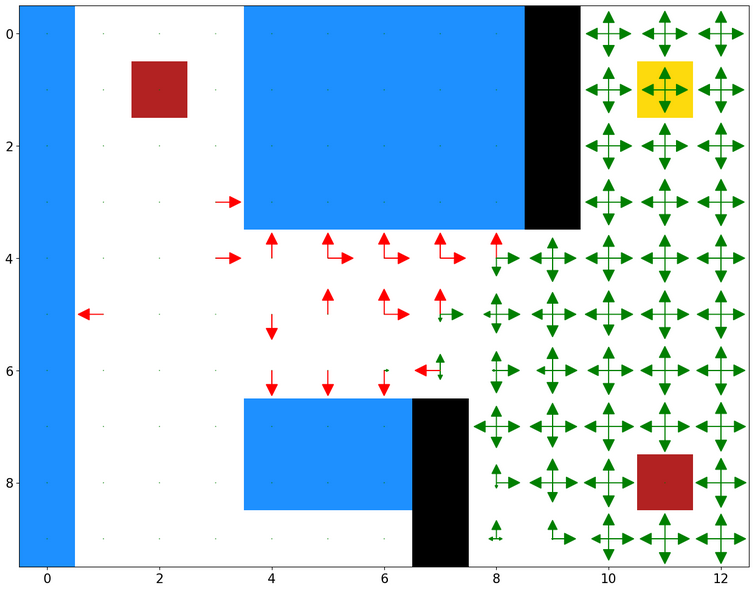
\includegraphics[width=0.9\textwidth]{3 Q plot.png}
  \caption{  num episodes = 5000, $\eta$= 0.5, $\gamma$ = 1 - 0.01, $\epsilon$ = 0.5}
\end{minipage}%
\begin{minipage}{.32\textwidth}
  \centering
  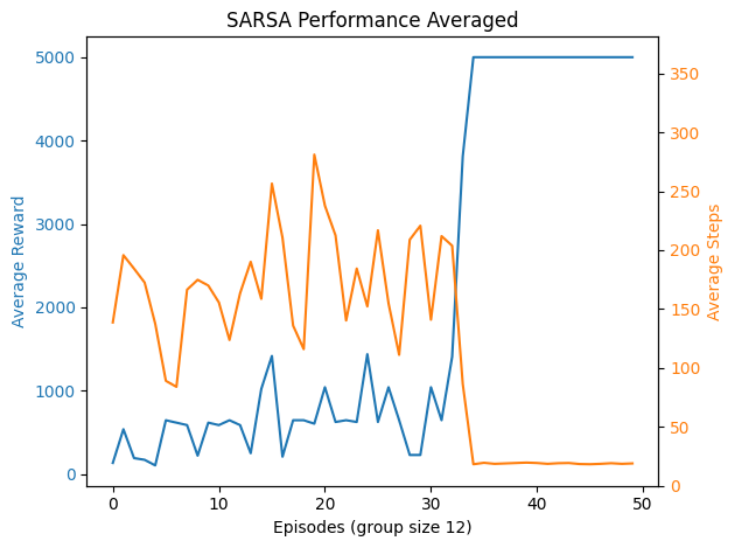
\includegraphics[width=1\textwidth]{10 performance plot.png}
\end{minipage}
\end{wrapfigure}

The same algorithm and parameters didn’t work as well on the 2 reward environment, struggling to explore enough to find the higher reward and getting stuck in a local minima. 
\\ \\ \\ \\

\begin{wrapfigure}{l}{0.6\textwidth}
  \centering
\begin{minipage}{.28\textwidth}
  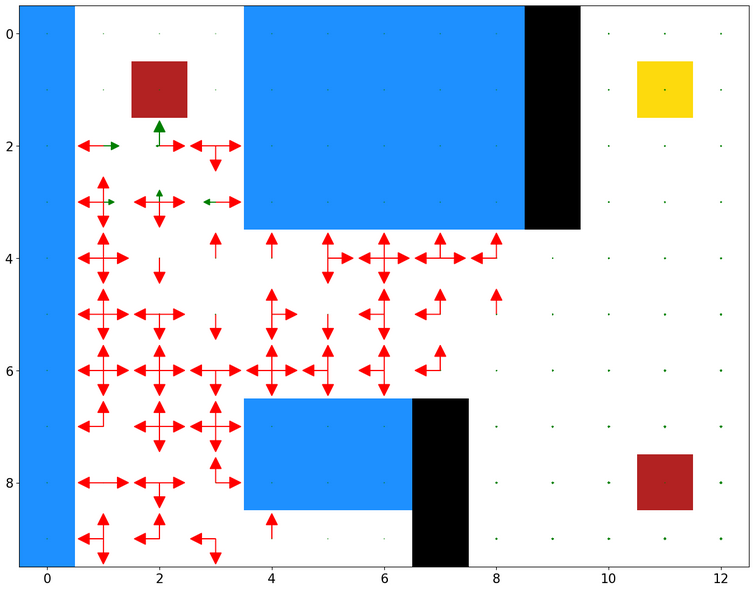
\includegraphics[width=0.9\textwidth]{4 Q plot.png}
  \caption{  num episodes = 5000, $\eta$= 0.5, $\gamma$ = 1 - 0.01, $\epsilon$ = 0.9}
\end{minipage}%
\begin{minipage}{.32\textwidth}
  \centering
  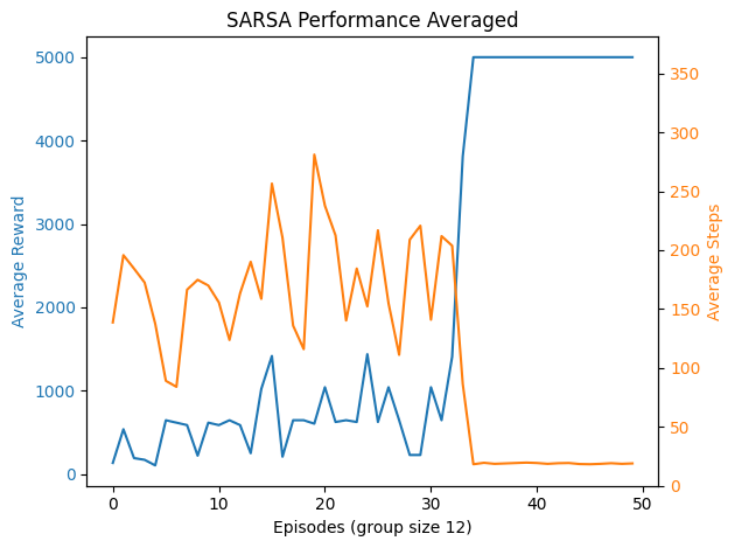
\includegraphics[width=1\textwidth]{10 performance plot.png}
\end{minipage}
\end{wrapfigure}

Increasing the $\epsilon$ value means the agent has a higher chance of exploring and so can get further on its random walk during the episode. This allows it to reach the far reward, but the high $\epsilon$ value also means that the agent follows the learned ideal direction less often and therefore will not necessarily make it back to the far reward to propagate the expected reward back towards the start. 
\\ \\ \\ \\

\begin{wrapfigure}{r}{0.6\textwidth}
  \centering
\begin{minipage}{.28\textwidth}
  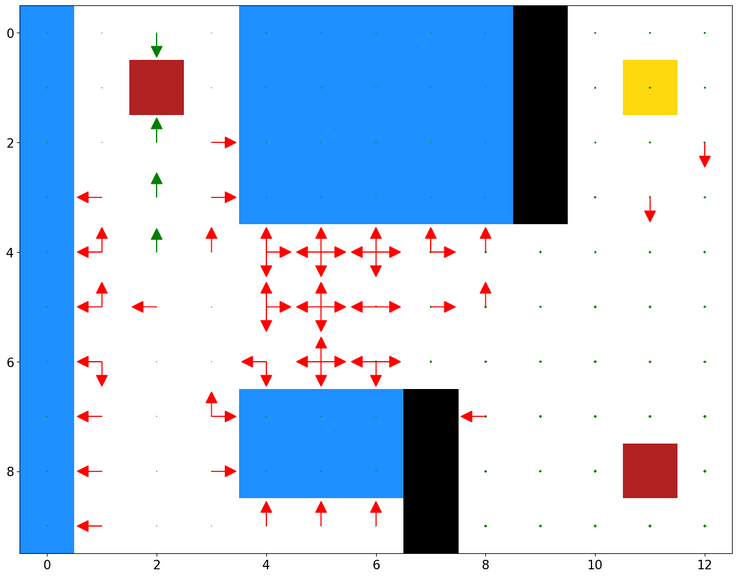
\includegraphics[width=0.9\textwidth]{5 Q plot.png}
  \caption{  num episodes = 5000, $\eta$= 0.98, $\gamma$ = 1 - 0.01, $\epsilon_0$ = 1, $\epsilon$ decay = 65}
\end{minipage}%
\begin{minipage}{.32\textwidth}
  \centering
  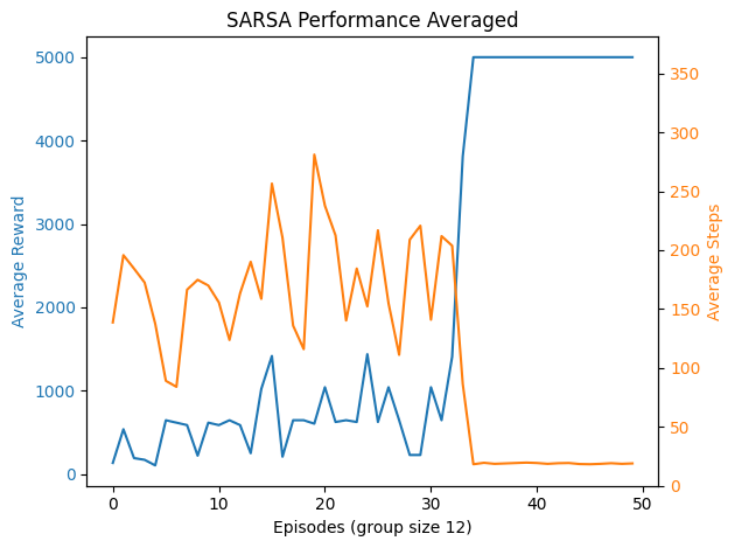
\includegraphics[width=1\textwidth]{10 performance plot.png}
\end{minipage}
\end{wrapfigure}

This would suggest that an $\epsilon$-schedule may improve the robot’s ability to learn Q. Using the formula $\epsilon$ = start * (decaytime - step) / decaytime, $\epsilon$ will decay over the episode. This should allow the agent to initially explore, and then over time will take greedy actions more and more frequently.
\\

This $\epsilon$ schedule did not improve the ability of the agent. This could be because many of the agents end up taking a random walk off of a cliff, ending the episode early and adding little new information to the system, and adding negative value to the states on the bridge which must be passed to collect the maximum reward. 
\\
\begin{wrapfigure}{l}{0.6\textwidth}
  \centering
\begin{minipage}{.28\textwidth}
  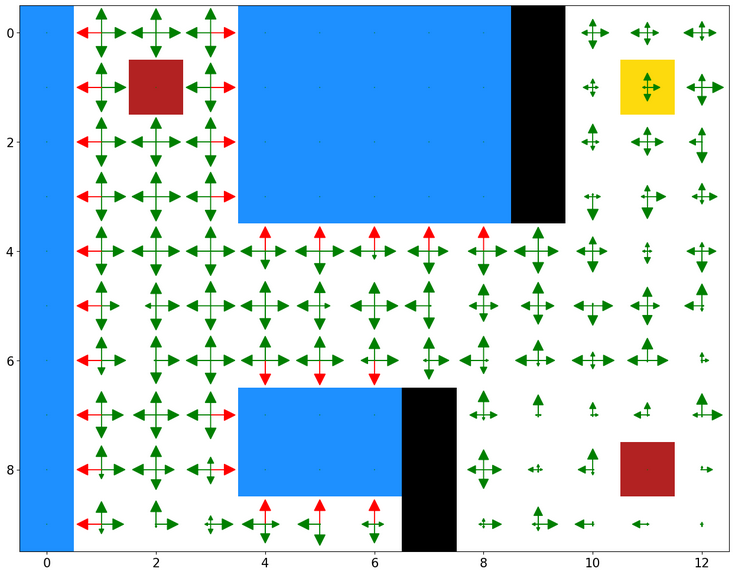
\includegraphics[width=0.9\textwidth]{11 Q plot.png}
  \caption{  num episodes = 4000, $\eta$= 0.98, $\gamma$ = 1 - 0.0001, $\epsilon_0$ = 1, $\epsilon$ decay = 250 }
\end{minipage}%
\begin{minipage}{.32\textwidth}
  \centering
  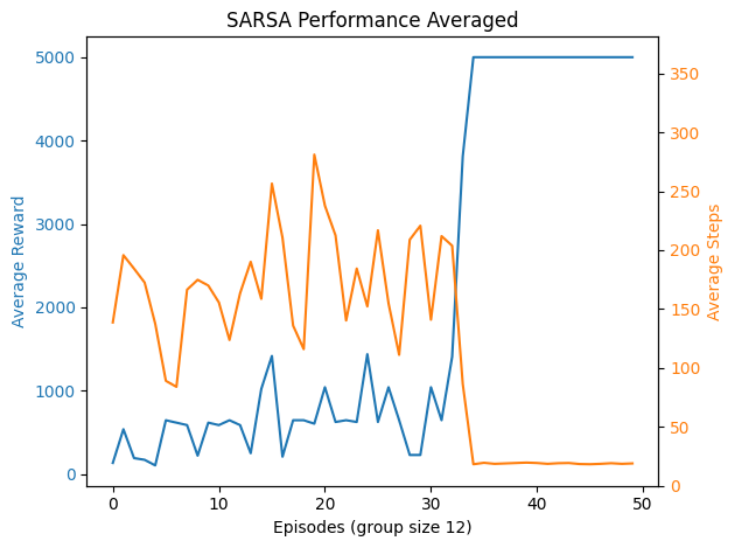
\includegraphics[width=1\textwidth]{10 performance plot.png}
\end{minipage}
\end{wrapfigure}

This can be solved by amending the epsilon-greedy policy, making sure it only randomly selects an action with negative expected value if there are no positive valued actions. We name this new policy epsilon-greedy-safe. 
\\ \\
Now that the passage is safe once the cliffs have been discovered, it is no longer given a low expected return. However, our agent is still not consistently achieving the best reward. This is because during every episode the agent is randomly moving for a lot of its lifespan. This means when it comes time to take its greedy actions, it may be attracted to the wrong reward or it may not make it to a reward before the maximum number of steps is up. 

\begin{wrapfigure}{l}{0.6\textwidth}
  \centering
\begin{minipage}{.28\textwidth}
  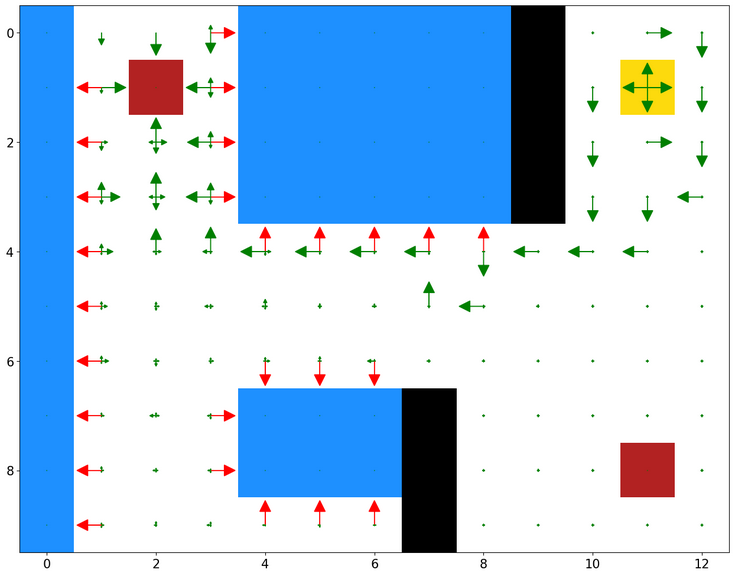
\includegraphics[width=0.9\textwidth]{10 Q plot.png}
  \caption{  num episodes = 600, $\eta$= 0.85, $\gamma$ = 1 - 0.0001, Stage 2 time = 400, Stage 2 $\epsilon$  =  0}
\end{minipage}%
\begin{minipage}{.32\textwidth}
  \centering
  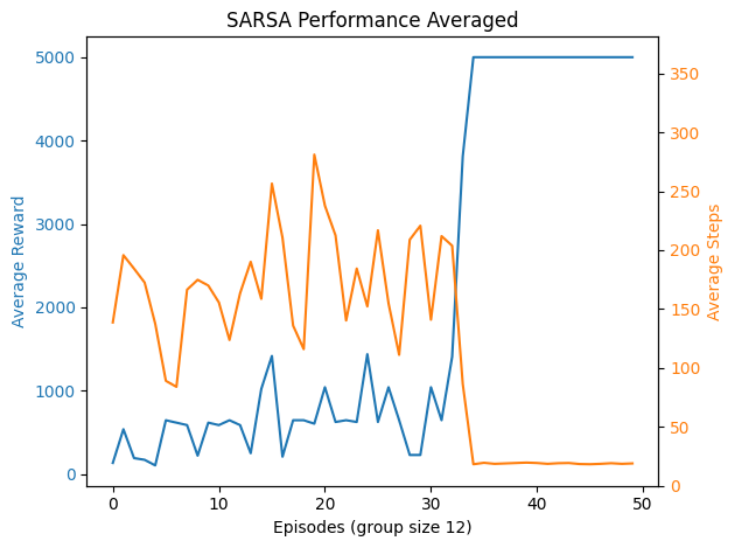
\includegraphics[width=1\textwidth]{10 performance plot.png}
\end{minipage}
\end{wrapfigure}
In order to fix this, we update the $\epsilon$-schedule to change based on the number of elapsed episodes instead of the step in each episode. We also change it to explore randomly for a fixed number of steps (safely), then act greedily. This means that after a fixed number of episodes, the agent will act according to the learned values and will achieve the maximum reward consistently.
\\
\begin{wrapfigure}{r}{0.6\textwidth}
  \centering
  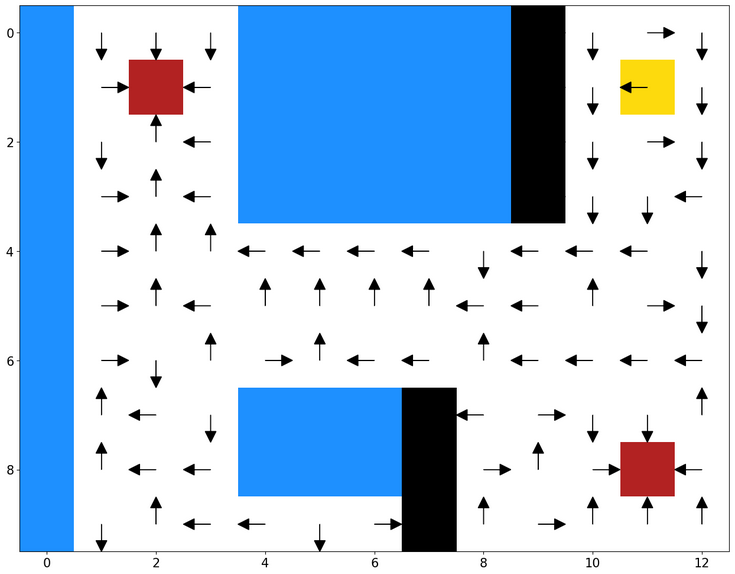
\includegraphics[width=0.6\textwidth]{10 policy.png}
  \caption{Figure 6's policy (best)}
\end{wrapfigure}

There are some issues with the learned policy. Namely, there are many infrequently visited states which don’t get a chance to learn about the newly updated values of its surrounding states. This causes suboptimal behaviour in these states, like cycling or in some cases receiving negative reward. This could potentially be fixed by implementing a second exploration epoch with a small value for $\epsilon$, so that the agent will still go towards the reward but will also explore.

\section{Conclusion}

In conclusion, the SERSA algorithm with a safe epsilon-greedy policy and $\epsilon$-schedule is adequate to successfully learn the gridworld environment, and to allow the agent to maximise total reward. Policy tuning and hyperparameter scheduling are very powerful tools that allow complicated scenarios to be modelled.









\end{document}
